\section{Mediciones y Experimentos}

Para poder realizar las mediciones utilizamos la instrucción de assembler \textit{rdtsc}. Con ella podemos obtener el valor de Time Stamp Counter (TSC) del procesador -un registro de 64 bits presente en todos los procesadores x86 desde los Pentium-, como este se incrementa en uno con cada ciclo del procesador podemos obtener la duración en cantidad de ticks de una llamada a una función calculando la diferencia de este registro al principio y al final de su ejecución. Ya que esta medida no es constante entre llamadas, por cada caso de test se realizaron 1000 llamadas y se las promedió utilizando el framework provisto por la cátedra. Para lidiar con los posibles outliers se calculó una media 10\% podada. Otros detalles de las mediciones se dan específicamente por cada experimento producido.

\subsection{Performance}

Nos propusimos observar el crecimiento en la cantidad de ciclos por llamada de cada función a medida que crecía el tamaño del archivo de entrada. Para esto utilizamos la imagen de Lena con tamaños de 16x16 píxeles hasta 1024x1024 en incrementos de a 8 píxeles por lado -para el filtro Blit las mediciones arrancaron con imágenes de 128x128 dadas las restricciones del filtro-. El objetivo de estos tests es comparar la performance de la implementación de cada filtro en un lenguaje de alto nivel como C y en uno de nivel más bajo como Assembler. Sabemos que la programación en bajo nivel provee poca -o ninguna- abstracción del set de instrucciones de una arquitectura, debido a esta cercanía del código con el procesador podríamos esperar que la ejecución sea más rápida y que fuese más eficiente en el uso de la memoria. Por el lado del código en C, hicimos las mediciones compilando con los flags O0 y O3 para observar en mayor detalle las variaciones en performance que introducen las optimizaciones del compilador.

A excepción de Temperature, en todos los resultados obtenidos observamos que nuestra implementación en ASM requirió menos ciclos de reloj que su contraparte en C en cualquiera de sus variantes. Sin embargo, en algunos filtros la diferencia fue menor que en otras. Las diferencias más notorias se dieron en los filtros Ondas y Edge, encontrando las menores diferencias en Monocromatizar y Temperature. Al mismo tiempo observamos diferencias significativos entre compilar el código en C usando los flags O0 y O3, donde encontramos que no utilizar optimizaciones (el flag O0) es la opción que más ciclos de reloj demora por llamada. 

Las diferencias registradas en cada implementación son coherentes con el diseño de los algoritmos dadas las posibilidades de cada paradigma de programación: mientras que en los casos de la programación en alto nivel con C toda la programación la realizamos secuencialmente procesando de a un píxel, en bajo nivel con ASM podemos procesar múltiples píxeles con pocas instrucciones SIMD, acortando significativamente la cantidad de ciclos. El grado de mejora entre una implementación está relacionado con el provecho que se haga de las ventajas que ofrece la paralelización de los datos, comparando con la compilación O0 -sin optimizaciones- es grande en todos los casos, sin embargo al introducir las optimizaciones con O3 el desempeño se acerca mucho al del ASM. Como contracara de esto debemos resaltar que no poseemos toda la información de cómo funciona exactamente el compilador a este nivel y con esas opciones, por lo que perdemos algo del control que tenemos programando puramente en C sin optimizar o en ASM.

\begin{wrapfigure}{r}{0.3\textwidth}
	\centering
	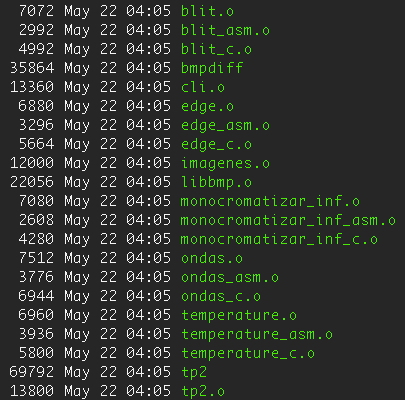
\includegraphics[width=0.3\textwidth]{imagenes/testperformance/sizes.png}
\end{wrapfigure}

Observamos que el código C optimizado con O3 funcionó mejor que nuestra implementación en ASM para Temperature, asimismo en Ondas sucedió lo contrario. En casos como Monocromatizar y Blit las diferencias fueron menores, probablemente porque el código mismo no tiene grandes saltos condicionales ni cálculos de punto flotante y al ser un simple loop, el código en C puede descomponer este loop y ganar algo de performance sobre el ASM -donde si bien levantamos de a 4 píxeles, tenemos mucho saltos por los ciclos-, este caso será investigado en un experimento posterior.

También podemos apreciar la diferencia en bytes de los archivos objeto producidos por los compiladores (primera columan de la imagen a la derecha). En todos los casos los archivos generados por GCC son más pesados que los ensamblados por NASM, pesando estos últimos entre un 55\% y un 65\% lo que pesan sus pares en C.

Como ventaja innegable que tiene C por sobre Assembly, o la de cualquier lenguaje de alto nivel por sobre uno de bajo nivel, es la facilidad de uso y debuggeo, su legibilidad, portabilidad, etc. Un ejemplo de esta diferencia es la cantidad de líneas de código que requiere cada algoritmo según el tipo de lenguaje utilizado, llegando nuestras implementaciones en ASM a requerir entre 2 y 5 veces la cantidad de líneas que ocupan en C.

A continuación están los gráficos correspondientes a los filtros y sus mediciones de performance. A la izquierda en escala lineal y a la derecha en escala logarítmica.

\begin{center}
	\begin{tabular}{cccc}
	  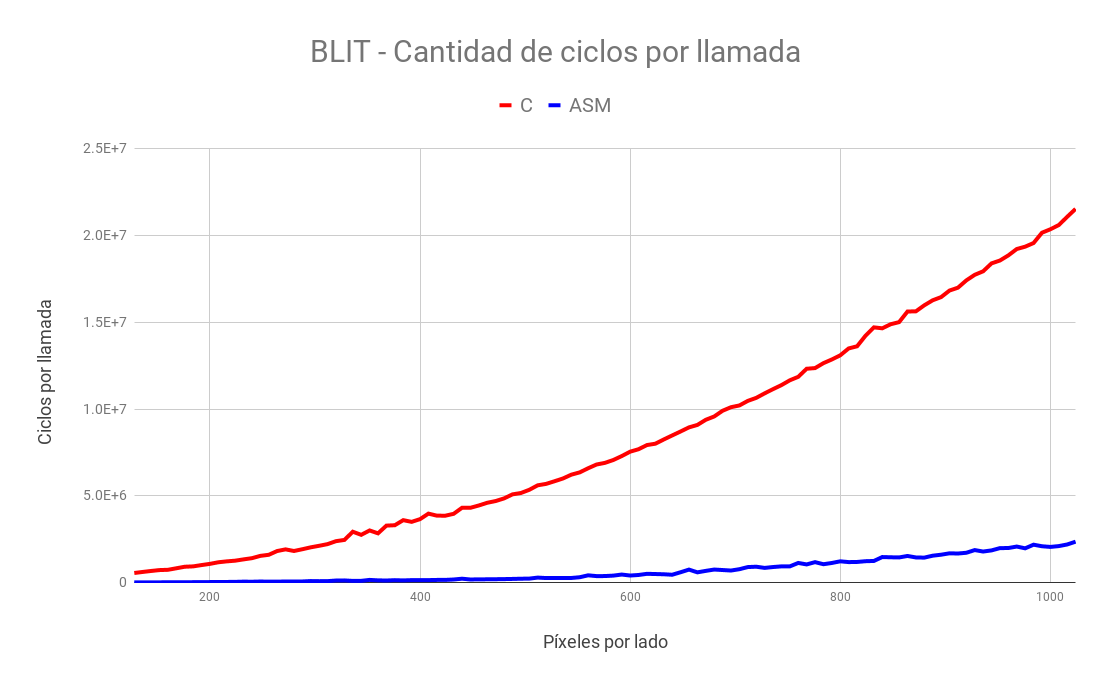
\includegraphics[width=0.45\textwidth]{imagenes/testperformance/BLITperformance.png} &
	  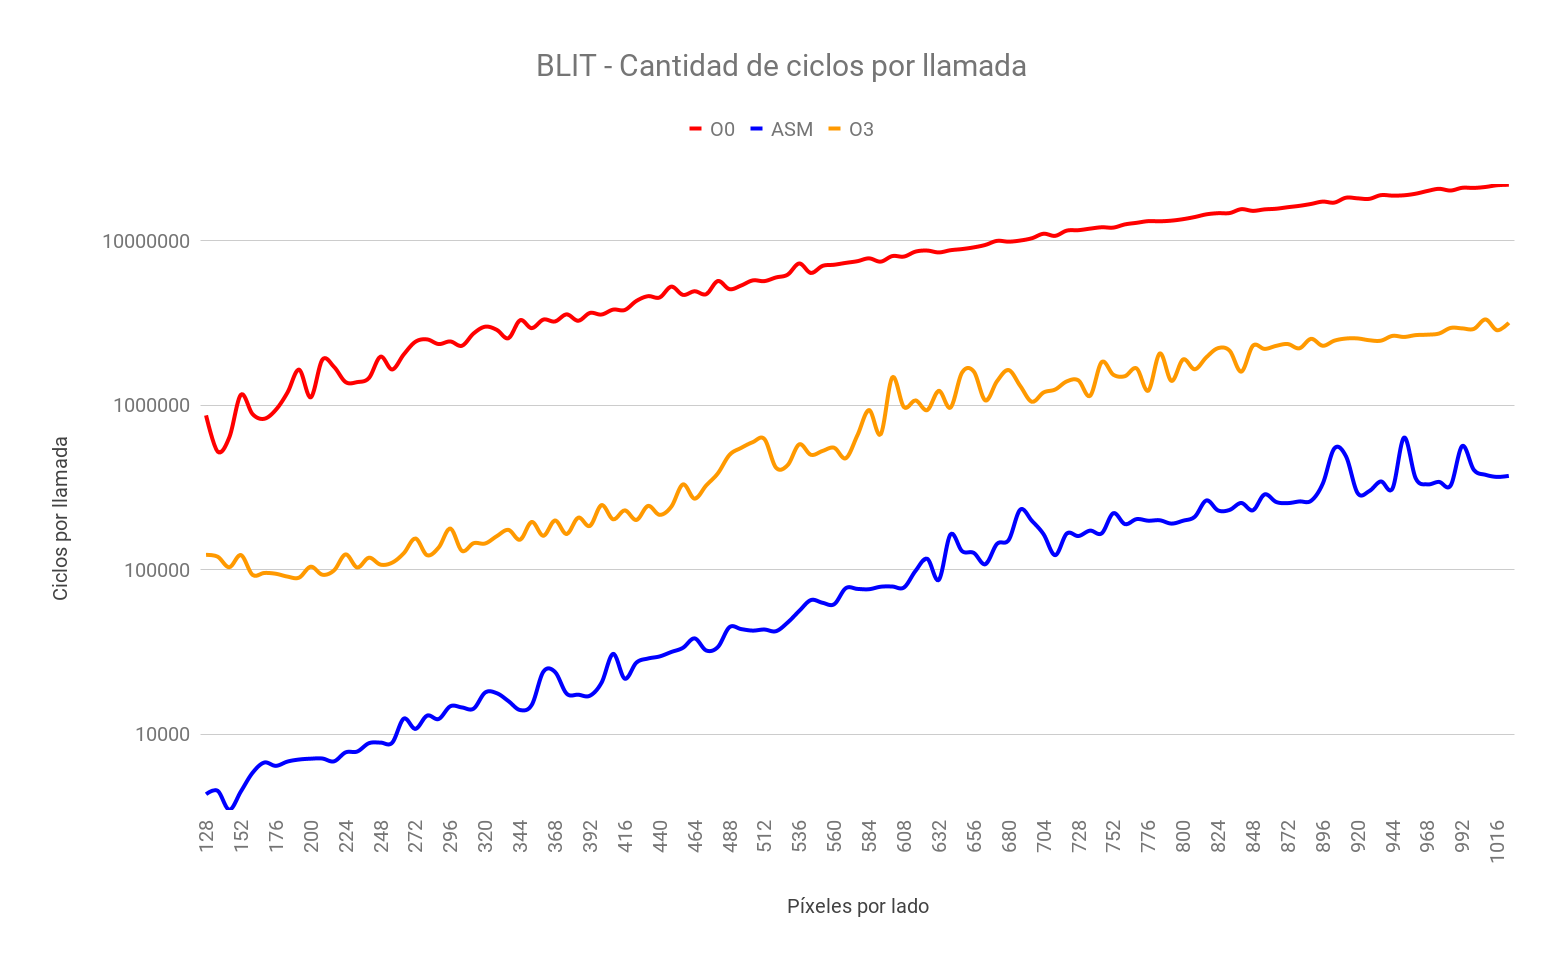
\includegraphics[width=0.45\textwidth]{imagenes/testperformance/BLITperformanceLOG.png} \\
	  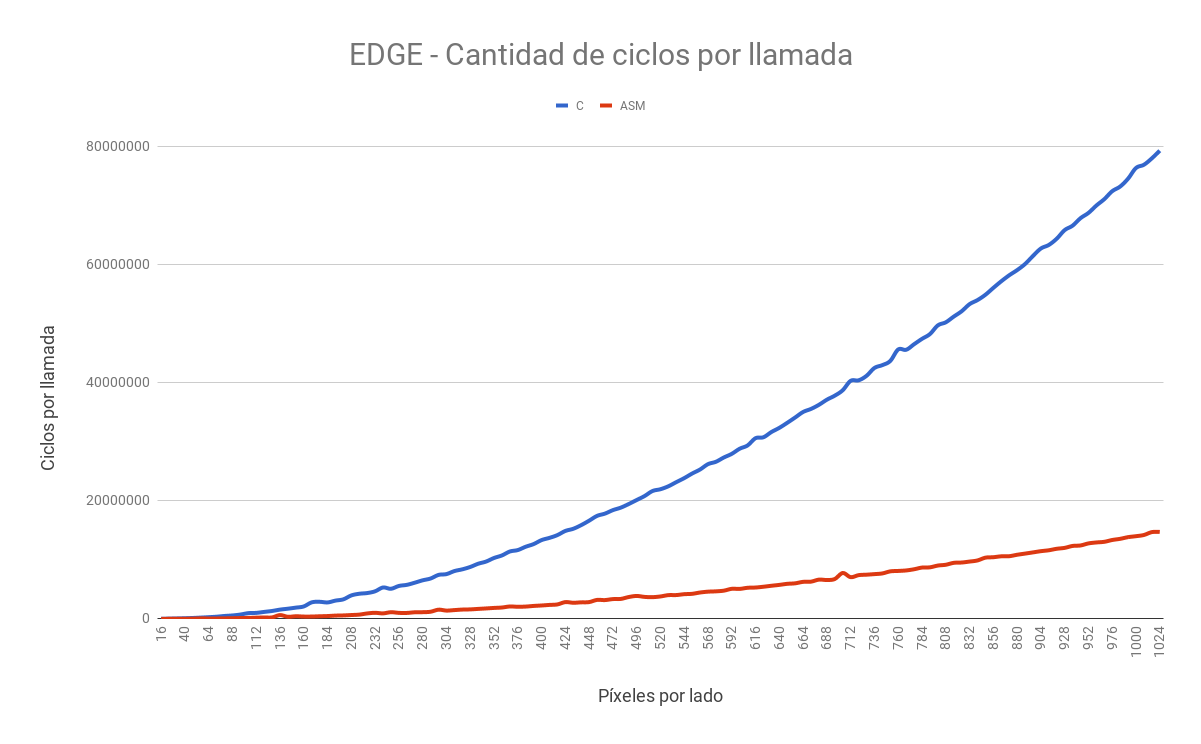
\includegraphics[width=0.45\textwidth]{imagenes/testperformance/EDGEperformanceLIN.png} &
	  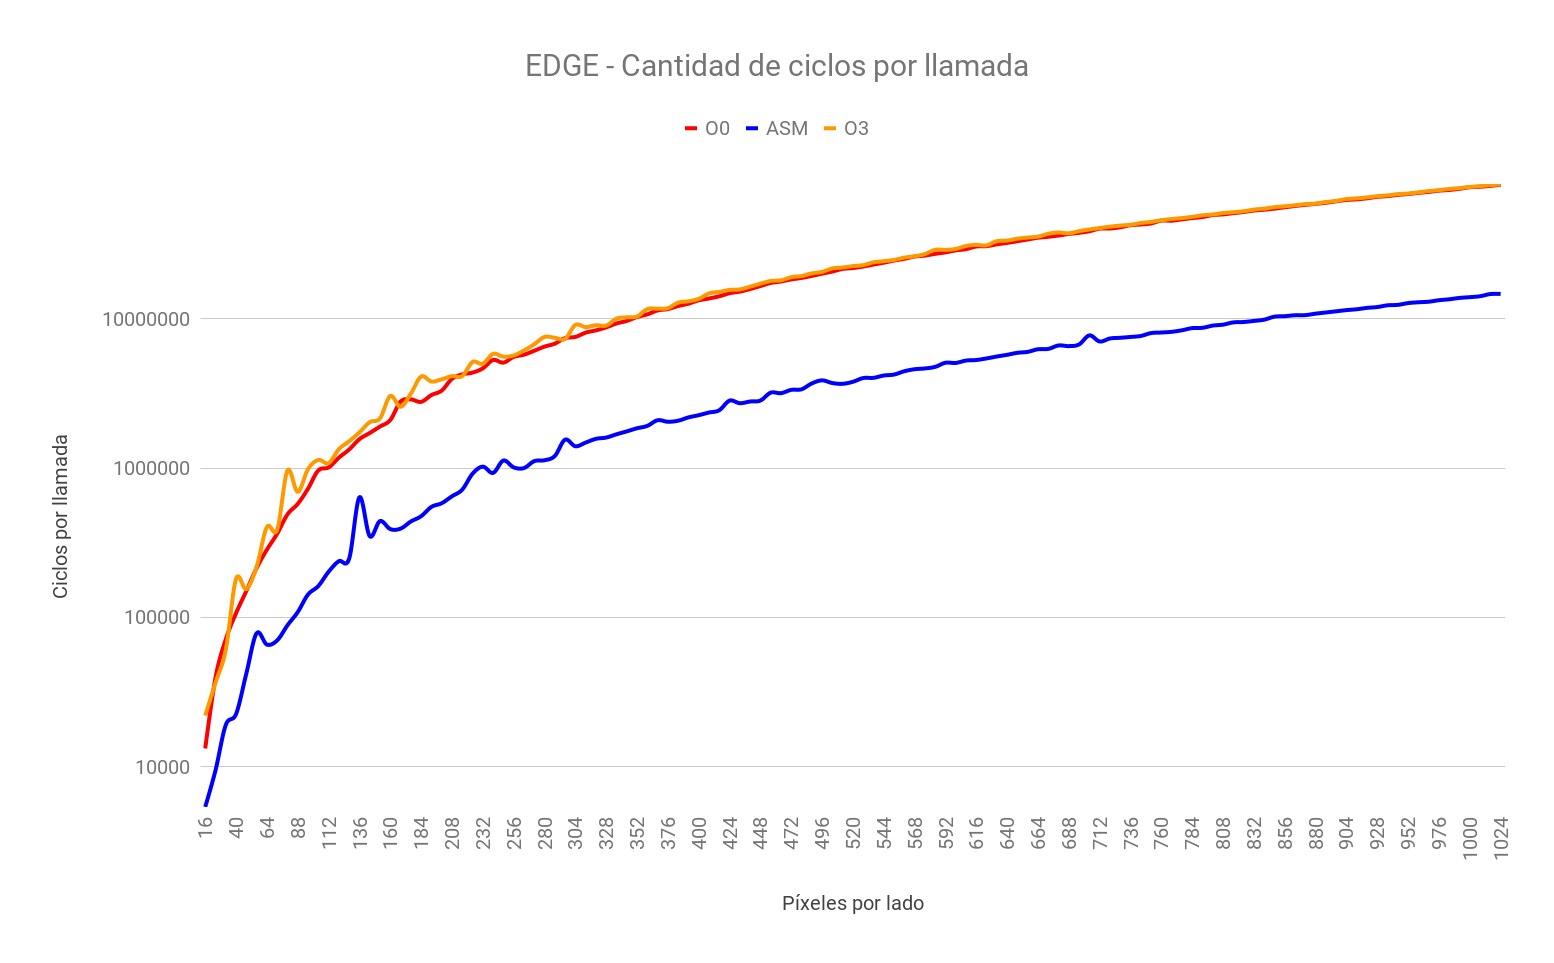
\includegraphics[width=0.45\textwidth]{imagenes/testperformance/EDGEperformanceLOG.png} \\
	  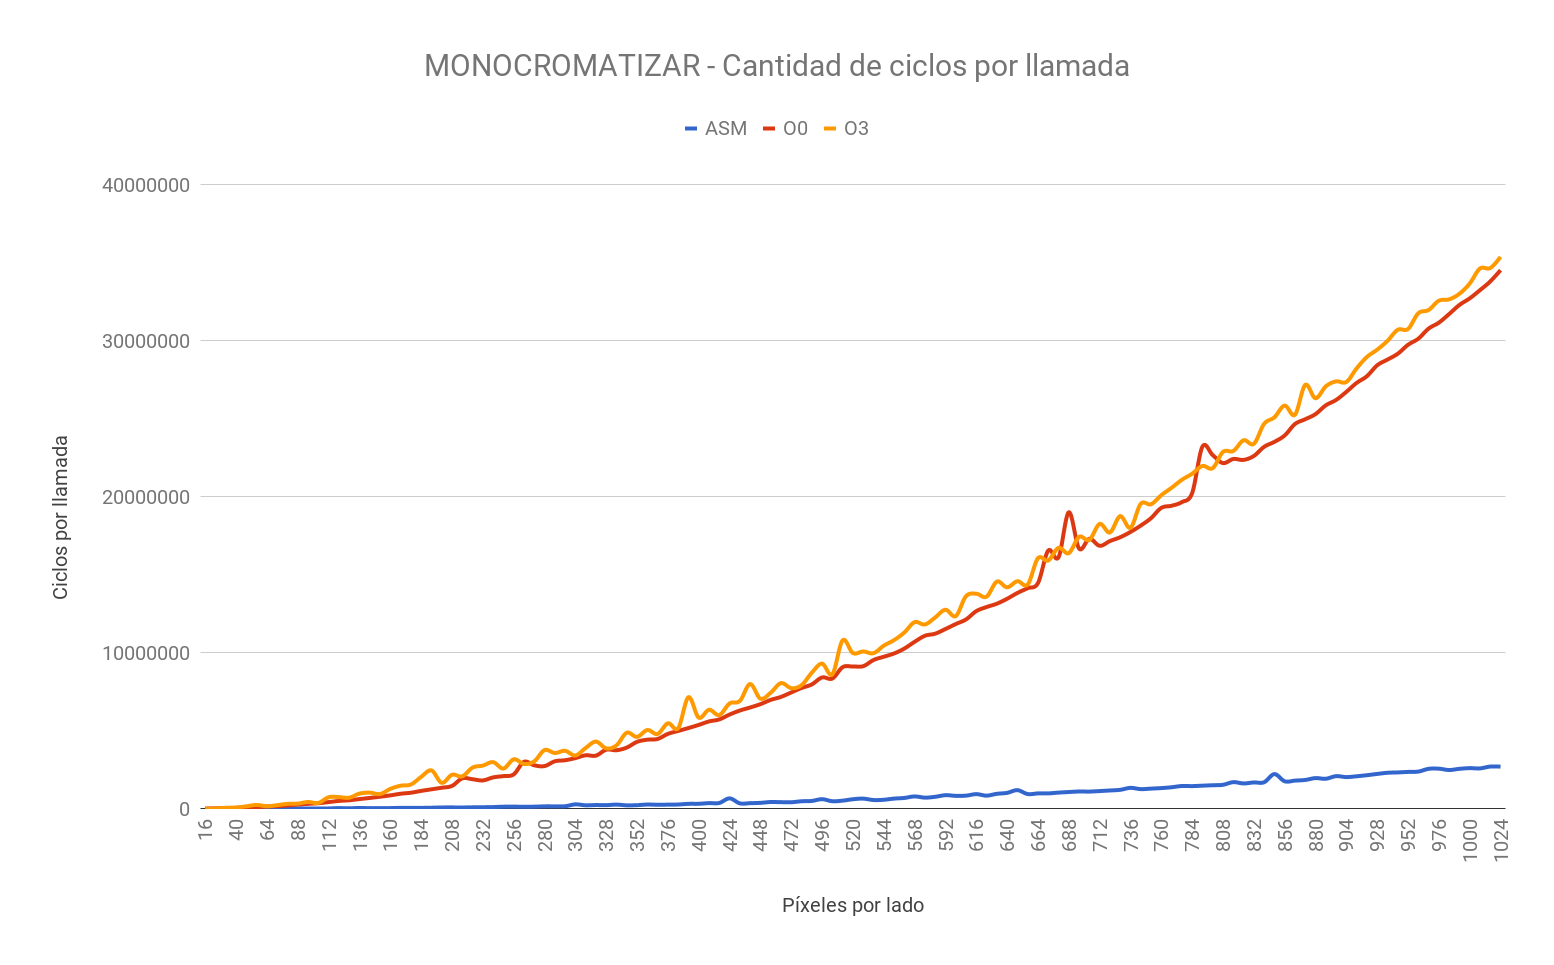
\includegraphics[width=0.45\textwidth]{imagenes/testperformance/MONOperformanceLIN.png} &
	  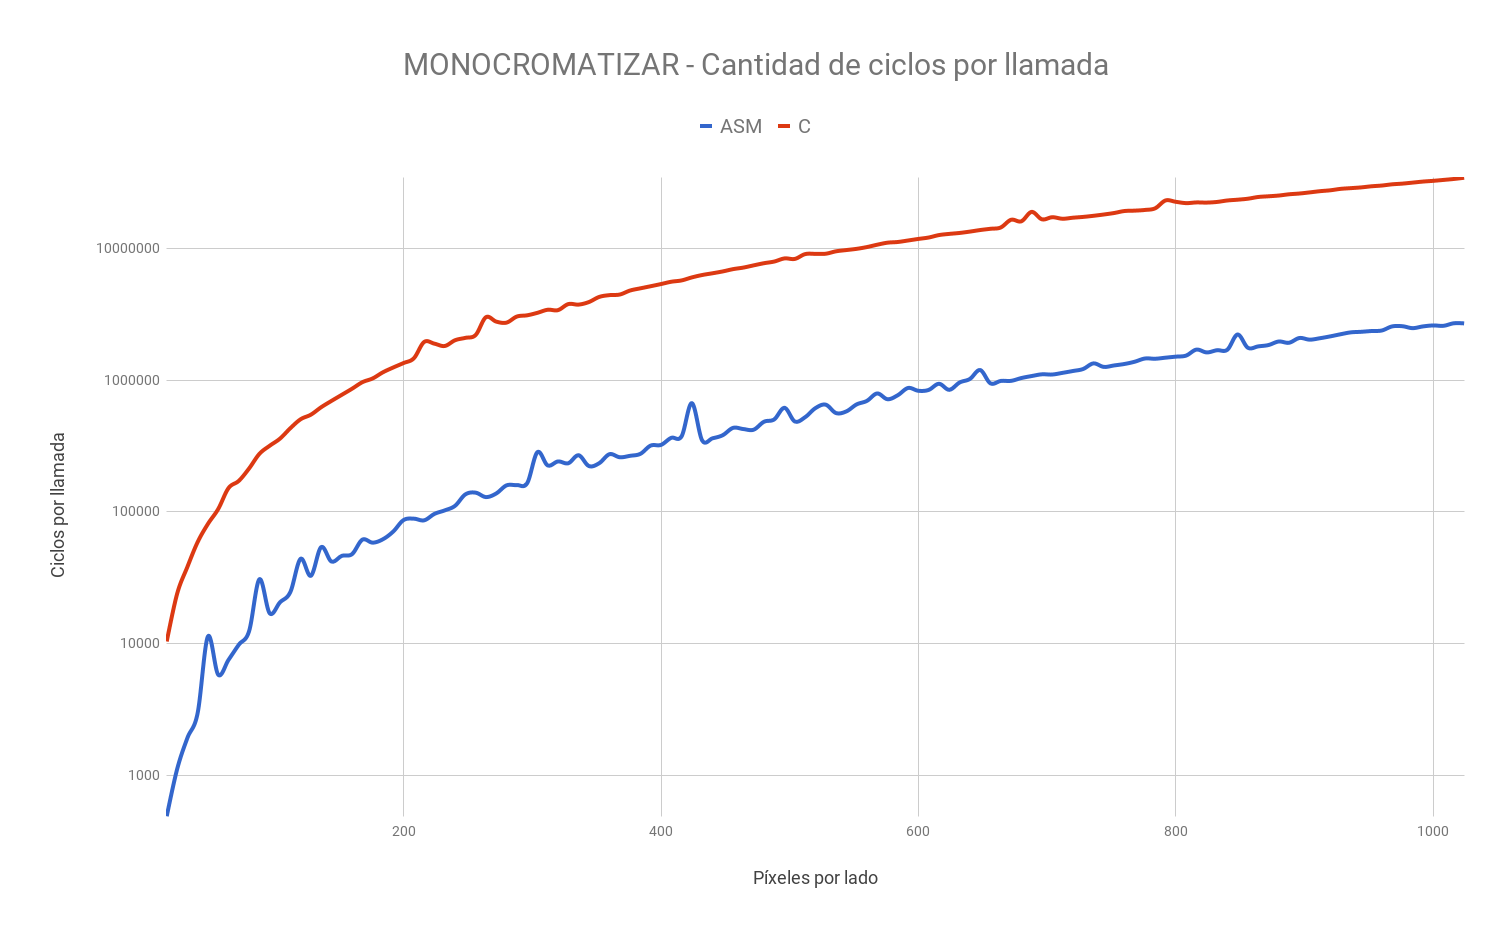
\includegraphics[width=0.45\textwidth]{imagenes/testperformance/MONOperformanceLOG.png} \\
	  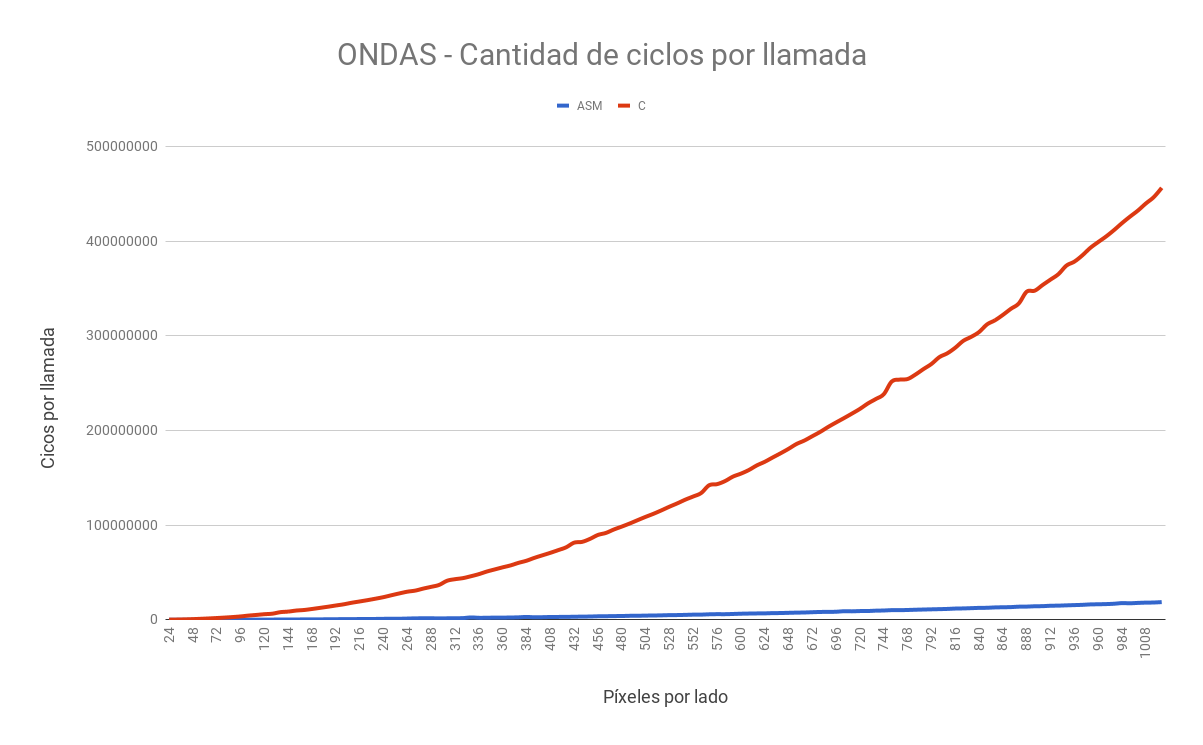
\includegraphics[width=0.45\textwidth]{imagenes/testperformance/ONDASperformanceLIN.png} &
	  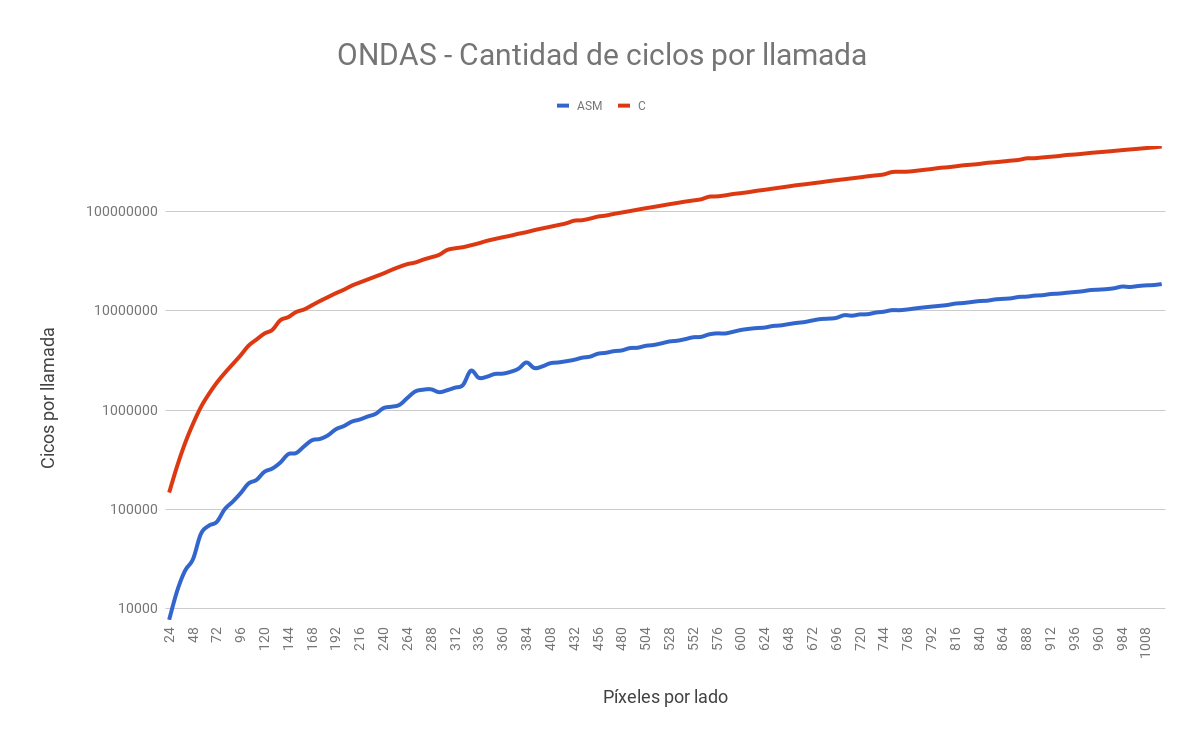
\includegraphics[width=0.45\textwidth]{imagenes/testperformance/ONDASperformanceLOG.png} \\
	\end{tabular}
\end{center}

\begin{center}
	\begin{tabular}{cccc}
	  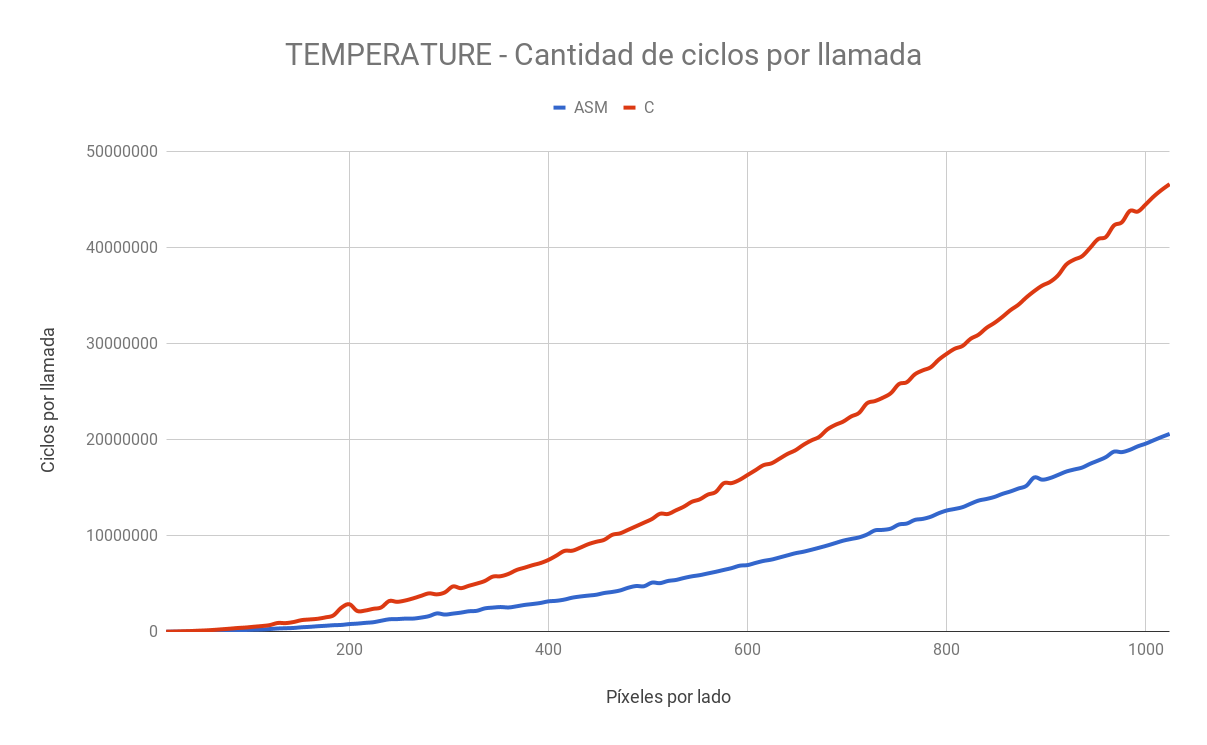
\includegraphics[width=0.45\textwidth]{imagenes/testperformance/TEMPperformance.png} &
	  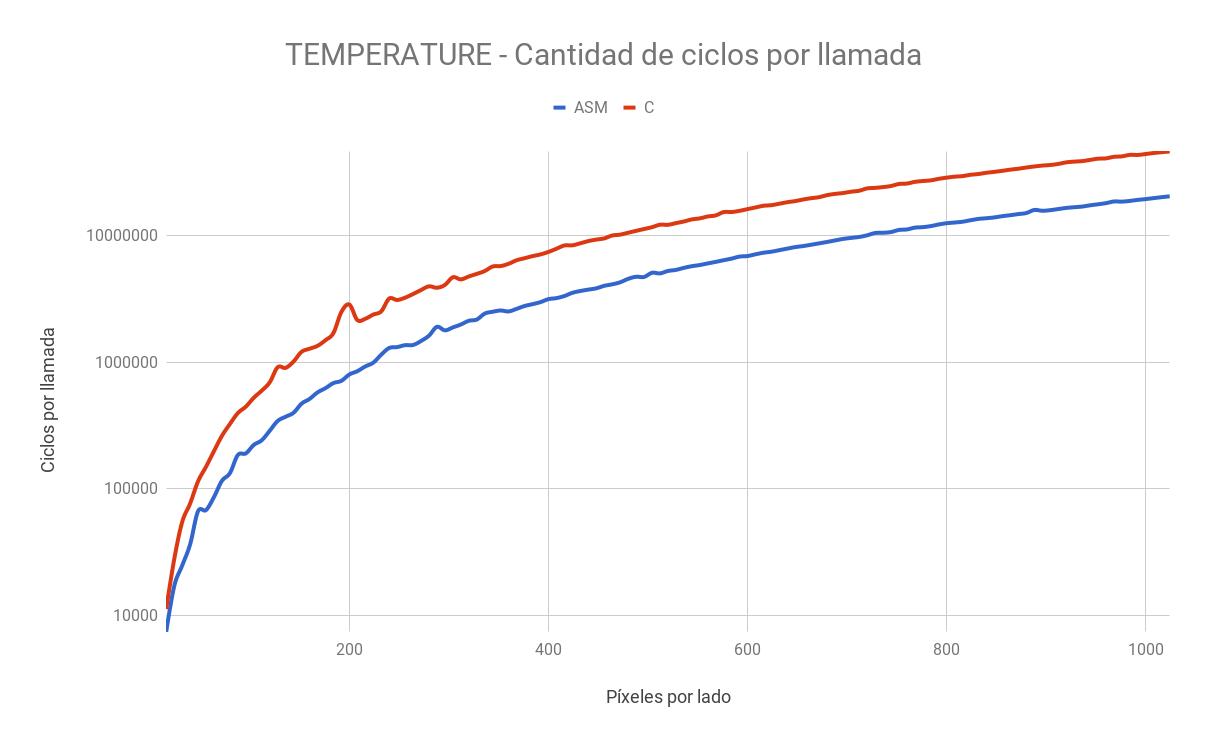
\includegraphics[width=0.45\textwidth]{imagenes/testperformance/TEMPperformanceLOG.png} \\
	\end{tabular}
   \end{center}

\subsection{SIMD vs. SISD}

En la misma línea del experimento anterior quisimos evaluar las diferencias de tiempo entre el mismo algoritmo implementado en C (sin optimizaciones), en ASM usando instrucciones SISD y en ASM con SIMD. La reescritura del código utilizando instrucciones SISD requirió 60 líneas de código, usando SIMD 30, y con C apenas 10; el tamaño de los archivos objeto pesó 2592B en SISD, 2608B en SIMD y 4280B en C.

\begin{center}

	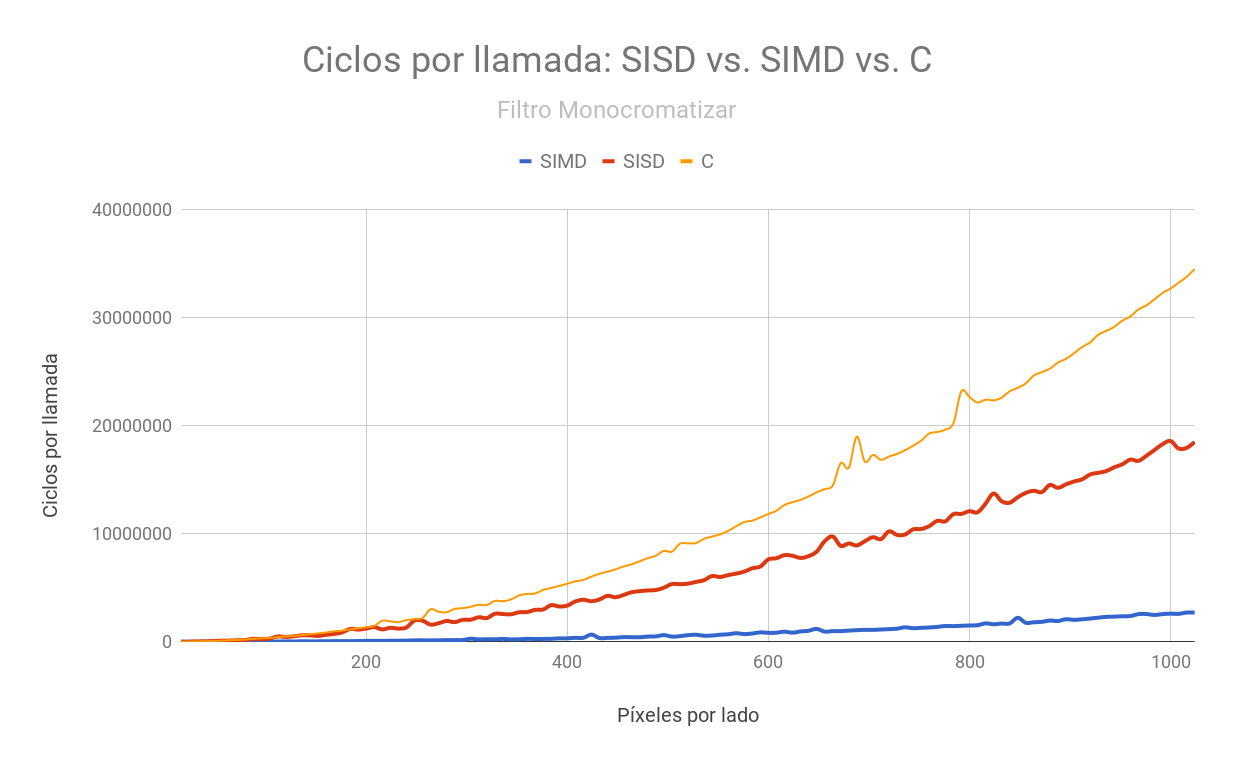
\includegraphics[width=0.9\textwidth]{imagenes/simdsisd/SIMDvsSISDvsClin.png} \\
	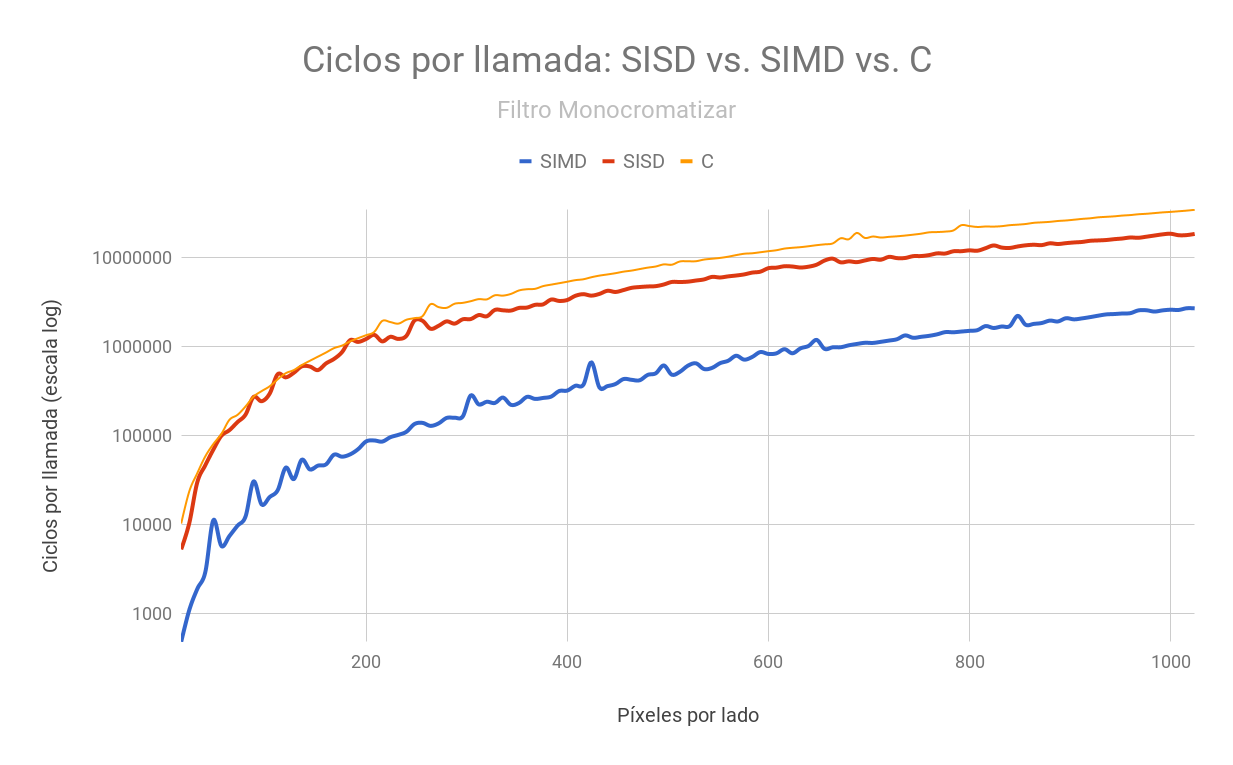
\includegraphics[width=0.9\textwidth]{imagenes/simdsisd/SIMDvsSISDvsClog.png}

\end{center}

Pudimos apreciar como las instrucciones SIMD logran una superioridad en performance con respecto a la programación trabajando con datos secuencialmente. El mismo algoritmo implementado utilizando instrucciones SISD no logró imponerse sobre C para imagenes pequeñas -por debajo de los 256 píxeles por lado-, aunque sí lo logró para imagenes de mayor tamaño. En este caso el beneficio de trabajar en ASM puede verse opacado por la facilidad de la programación en C si no se utilizan las instrucciones SIMD. Sin embargo de mantenerse este crecimiento en la cantidad de llamadas para cada implementación, C sigue perdiendo cuando es más exigido.

\newpage
\subsection{Branch Prediction}

Un predictor de saltos es un circuito digital que intenta adivinar por qué rama de una estructura condicional va a continuar la ejecución de un programa antes de que se lo sepa definitivamente. El objetivo del predictor de saltos es mejorar el flujo del pipeline. En el presente experimento nos propusimos intentar forzar al predictor de saltos a funcionar en escenarios donde pueda predecir fácilmente las instrucciones siguientes y es escenarios donde no lo pueda lograr. Para esto trabajamos con el filtro Temperature en C exclusivamente (compilando con O0 y O3) ya que dada la lógica del algoritmo este filtro es el mejor ejemplo para hacer estas pruebas, además los compiladores son los responsables de armar los loops de modo de usar las instrucciones en función del branch prediction. Recordemos la lógica condicional del filtro:
\begin{center}
	\begin{displaymath}
	\mathsf{dst}_{(i,j)}<r,g,b> = \left\{
	\begin{array}{l l}
				<0,0, 128 + t \cdot 4> & \text{si }t < 32\\
				<0, (t - 32) \cdot 4, 255> & \text{si }32 \le t < 96\\
				<(t-96) \cdot 4, 255, 255 - (t-96) \cdot 4> & \text{si }96 \le t < 160\\
				<255, 255 - (t - 160) \cdot 4, 0> & \text{si }160 \le t < 224\\
				<255 - (t - 224) \cdot 4, 0 , 0> & \text{si no} \\
	\end{array}
	\right.
	\end{displaymath}
	\end{center}

Para caer en cada una de estas condiciones utilizamos varias imágenes, con tamaños de 16x16 píxeles a 1024x1024:

\begin{itemize}
	\item Una imagen complemente negra, (0,0,0) en todos sus píxeles.
	\item Una imagen complemente blanca, (255,255,255) en todos sus píxeles.
	\item Una imagen con un patrón donde un píxel entra a la primera rama del condicional, el segundo píxel a la segunda rama, el tercero a la tercera etc... (incluímos la imagen abajo a la izquierda)
	\item Una imagen con ruido, donde todos los píxeles fueron generados al azar utilizando un filtro en GIMP. (Abajo a la derecha).
\end{itemize}

Las imagenes utilizadas:

\begin{center}
	\begin{tabular}{cccc}
	  
\includegraphics[width=0.45\textwidth]{imagenes/antiTEMP.jpg} &
	  
\includegraphics[width=0.45\textwidth]{imagenes/random.jpg} \\
	\end{tabular}
   \end{center}

\begin{center}

	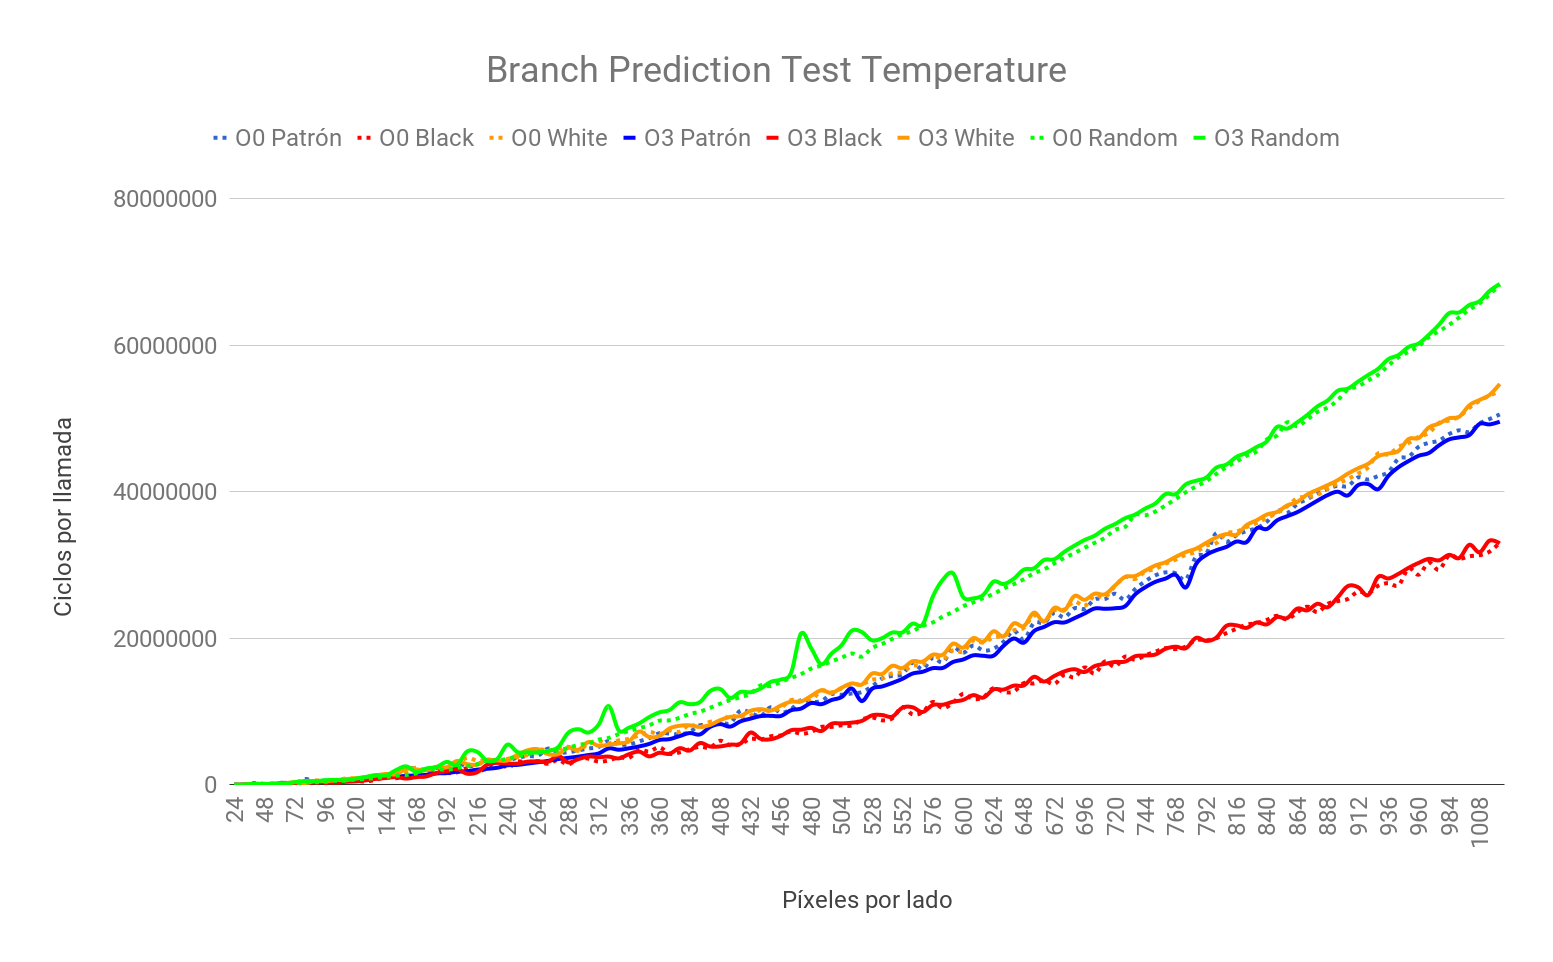
\includegraphics[width=0.9\textwidth]{imagenes/branchprediction/branchpredictionLIN.png} \\
	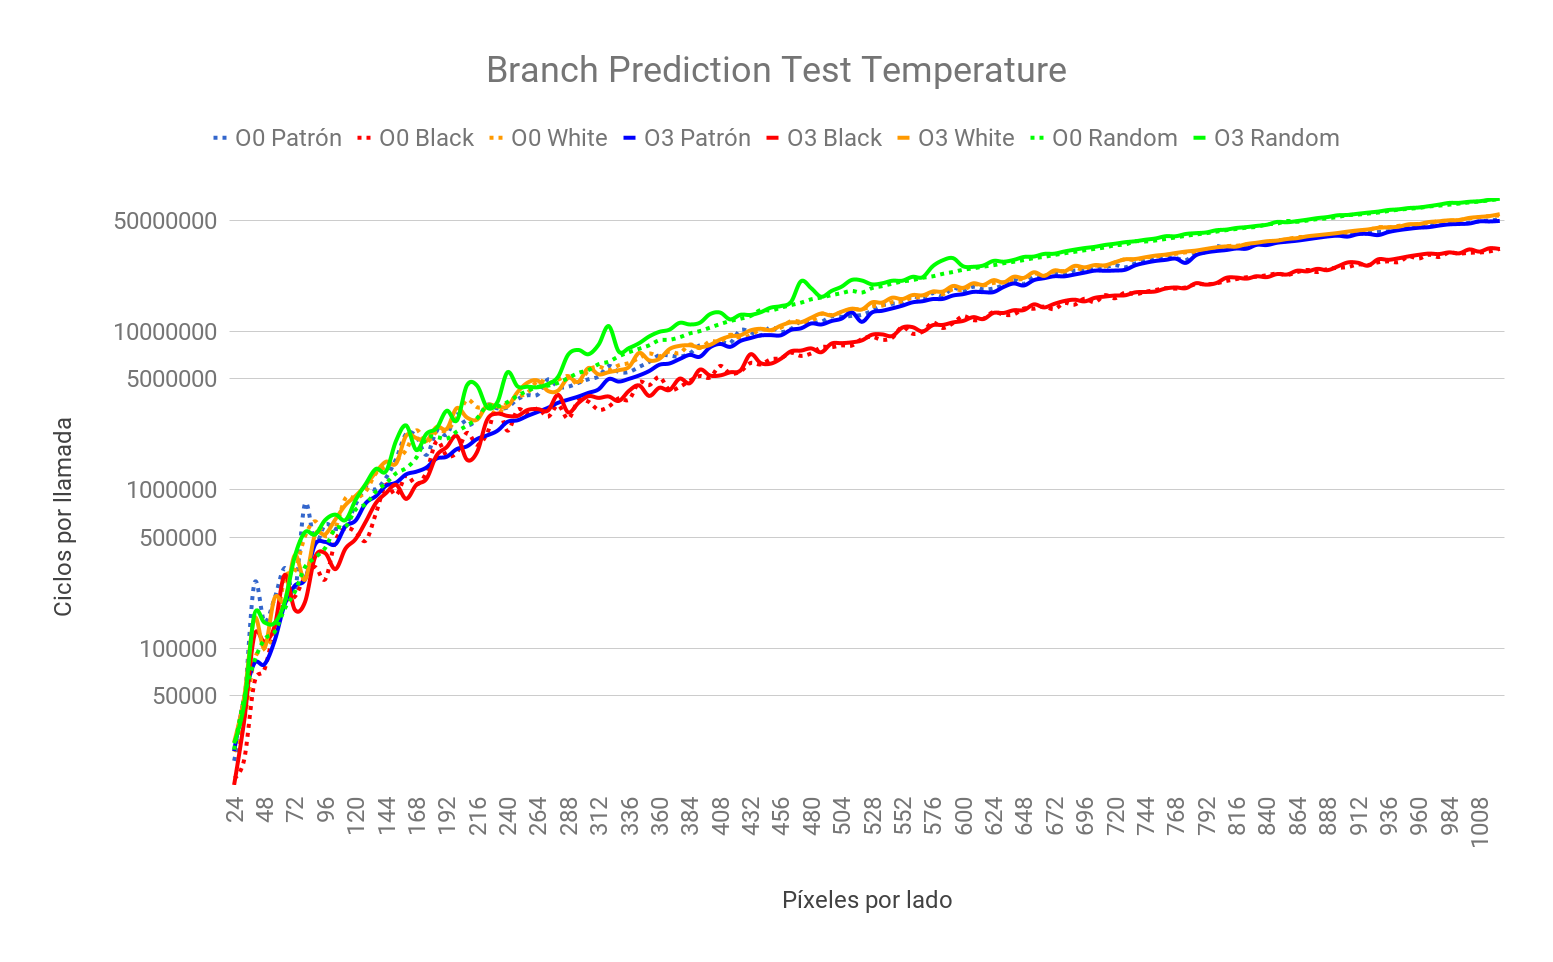
\includegraphics[width=0.9\textwidth]{imagenes/branchprediction/branchpredictionLOG.png}

\end{center}

A partir de los resultados pudimos observar lo siguiente: el predictor de saltos pudo mejorar los tiempos de ejecución del programa en la imagen negra para todos los casos a partir de un tamaño de 312 píxeles por lado; no hubo diferencias sustanciales entre las imagenes blancas y las que incluyen el patrón, efectivamente las imagenes blancas demoraron unos ciclos más que las del patrón, posiblemente porque tiene que evaluar todas las condiciones antes de caer en el caso correcto, mientras que para el patrón algunos píxeles entran en las primeras ramas del condicional y no hace falta seguir evaluando; finalmente para el caso de la imagen con ruido los ciclos de llamada fueron mucho mayores que para el resto, incluso presentan una tasa crecimiento mayor, especialmente a partir de los 400 píxeles por lado. También volvemos a notar que las optimizaciones O3 introducen mejoras en rendimiento por sobre O0 en todos los casos probados.

\newpage
\subsection{Loop Unrolling}

Luego de verificar el impacto del branch pedictor procedimos a evaluar el impacto del loop unrolling con el filtro Monocromatizar en su implementación de ASM. El loop unrolling es una técncia que consiste en transformar un loop para intentar optimizar la ejecución de un programa a expensas del tamaño de su archivo binario. La ventaja de deshacer el loop y hacer una instrucción detrás de la otra es que se eliminan los branches que componen cualquier loop y desaparecen las penalizaciones relacionadas con estos obstáculos; sin embargo, dado que el procesador almacena en la caché las instrucciones a ejecutar, deberíamos notar una caída en performance cuando el código exceda el tamaño de la misma. Utilizamos la imagen de Lena con tamaño de 512x512 para estas pruebas. La macro utilizada corresponde al segmento de código en el que se levantan los píxeles de la imagen original, se calcula el máximo componente de cada uno y se escribe este valor los píxeles correspondientes de la imagen destino:

\begin{center}

	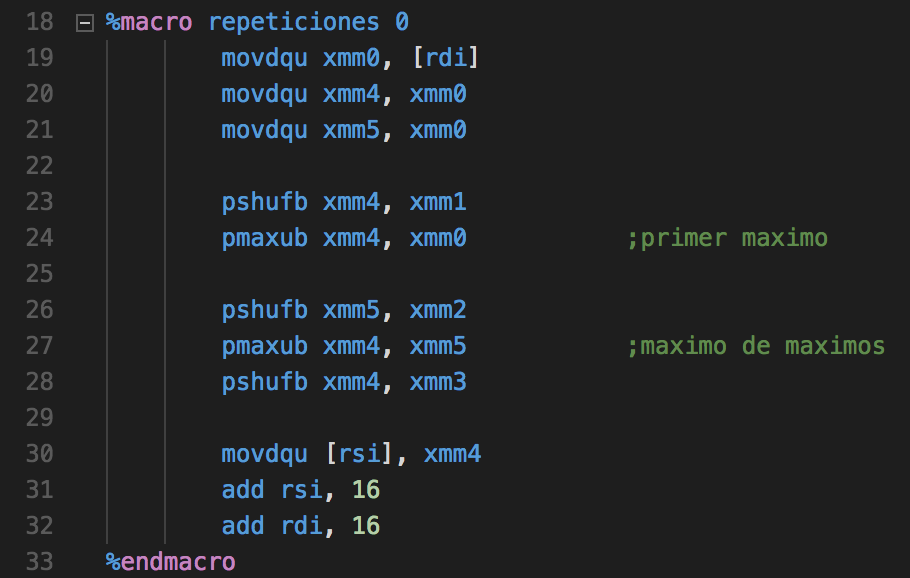
\includegraphics[width=0.45\textwidth]{imagenes/loopunrolling/macro.png}
	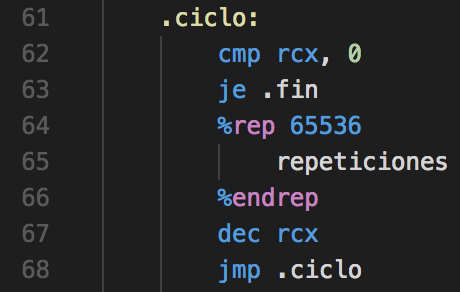
\includegraphics[width=0.45\textwidth]{imagenes/loopunrolling/reps.png}

\end{center}

Para la ejecución fuimos aumentando la cantidad de repeticiones que se hacían de la macro a medida que lo compensabamos disminuyendo la cantidad de loops que la contenían, o sea, en un extremo una repetición de la macro era ejecutada en un loop 65536 veces y en el otro una macro repetida 65536 veces era ejecutada una única vez, por ende, sin loop.

\begin{center}

	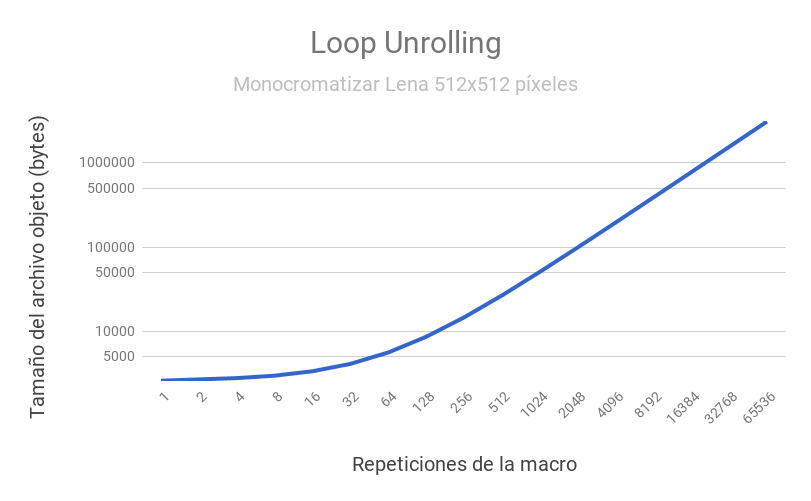
\includegraphics[width=0.9\textwidth]{imagenes/loopunrolling/size.png}

\end{center}

Como era de esperar el tamaño del binario aumentó con cada repetición de la macro. Sin hacer loop unrolling, el binario de nuestro filtro original ocupó apróximadamente 2000B, luego para poder procesar una imagen del mismo tamaño se descompuso el loop en 65536 repeticiones de la macro, lo cual llego al binario a pesar varios megas excediento el tamaño de la caché.

\begin{center}

	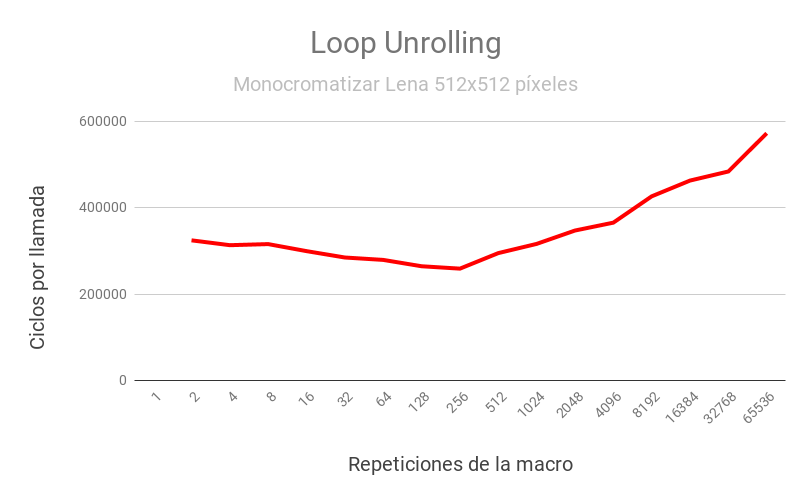
\includegraphics[width=0.9\textwidth]{imagenes/loopunrolling/time.png}

\end{center}

Notamos que hay leves mejoras cuando extendemos el loop hasta 256 repeticiones de la macro, a partir de este momento mientras descompongamos el loop en más repeticiones, más ciclos de procesador van a ser necesarios para terminar. Esto es coherente con lo expuesto anteriormente, a partir de cierto punto el binario es demasiado grande para la memoria caché y para ejecutar las instrucciones siguientes debe ir a buscar a memoria, provacando que el pipeline se detenga hasta que la próxima instrucción esté disponible e impactando negativamente en el desempeño del algoritmo.

% La forma de medir el rendimiento de nuestras implementaciones se realizará por medio de la toma de tiempos de ejecución del algoritmo (sea este el codigo version asembler o el codigo C). Como los tiempos de ejecución son muy pequeños, se utilizará uno de los contadores de performance que posee el procesador.
% La instrucción de assembler rdtsc permite obtener el valor del Time Stamp Counter (TSC) del procesador. Este registro se incrementa en uno con cada ciclo del procesador. Obteniendo la diferencia entre los contadores antes y después de la llamada a la función, podemos obtener la cantidad de ciclos de esa ejecución. Esta cantidad de ciclos no es siempre igual entre invocaciones de la función, ya que este registro es global del procesador y se ve afectado por una serie de factores. \newline

% Existen principalmente dos problemáticas a solucionar:
% 1). La ejecución puede ser interrumpida por el scheduler para realizar un cambio de contexto,
% esto implicará contar muchos más ciclos (outliers) que si nuestra función se ejecutara sin
% interrupciones.

% 2). Los procesadores modernos varían su frecuencia de reloj, por lo que la forma de medir
% ciclos cambiará dependiendo del estado del procesador.
% \newline

% \textbf{solucion 1):} Para evitar el problema de los ciclos outliers lo que hicimos fue,

% \begin{itemize}
% 	\item[Paso 1:] En nuestro caso hicimos 100 veces la medición de tiempo de nuestro algoritmo y guardarlo en un contenedor(podría ser un arreglo,lista, conjunto, diccionario,.., etc).
% 	\item[Paso 2:] Sacar la media, tambien conocido como promedio, ejemplito:
% 		\begin{center} $ Prom =\frac{x_1+x_2+...+x_{100}}{100}$ \end{center}
% 		Donde $x_i$ es la medición de tiempo de la medición número $i$, con $1 \leq i \leq 100$ 
% 	\item[Paso 3:] Calculamos la varianza: 			
% 				\begin{center}
% 					$Varianza = \sigma^2 = \frac{(x_1 - Prom)+ (x_2 - prom)+ ...+ (x_{100} - prom)}{100} $
% 				\end{center}
% 	\item[Paso 4:] Calculamos el desvio estandar,  $\sigma = \sqrt{Varianza}$
% 	\item[Paso 5:] Utilizando el desvio estandar y el promedio, puedo ver que medición es "buena"  \\ y cual no. Más formalmente una medicion es "buena" si cumple: 
% 					\begin{center}
% 					$Prom - \sigma \leq x_i \leq Prom + \sigma $. %%\newline
% 					\end{center}
% 	 Luego sumando las todas las mediciones  "buenas" \\ y dividiendalas por la cantidad de mediciones buenas, obtengo el "promedio bueno". Con esto amortiguaria la cantidad de outliers de mis mediciones. 			
% \end{itemize}

% \textbf{Observar:} Todo lo anterior sirve también para mas de 100 mediciones. \newline

% \textbf{Solucion 2):} La solución que planteamos para esto fue, ejecutar sólamente el algoritmo. Con esto queremos decir que la ejecución estara en el nivel más alto de privilegio de ejecución. Esto lo hacemos metiendonos en el sistema operativo (en este caso ubuntu 14.04), tocando el monitor de sistema para darle privilegio a la ejecución. Tambien evitamos interumpir la maquina de forma mecanica(osea humana).  
